\section{Grammatik} \label{sec:while-grammar}
Die Konzepte, welche in \cref{sec:while-konzepte} vorgestellt wurden, wurden in einer Form beschrieben, die für Menschen gut verständlich ist. Ein Computerprogramm, wie beispielsweise ein Compiler benötigt eine andere Form der Erklärung, wie der Aufbau eines Programmcodes auszusehen hat. Diese Erklärung erfolgt mithilfe von unterschiedlichen Grammatikregeln, welche in der sogenannten \ac{ebnf} aufgeschrieben werden. Ein Beispiel für zwei Grammatikregeln ist in \cref{lst:while-grammar-pred} zu sehen.

\begin{lstlisting}[language=c, caption=Zwei einfache Grammatikregel, label={lst:while-grammar-pred}]
	ID:    [a-zA-Z][a-zA-Z0-9]*;
	pred: 'pred' '(' ID ')' ';';
\end{lstlisting}

In der ersten Zeile ist zu sehen, wie eine \textbf{ID} aufgebaut sein muss, sie muss mit einem kleinen Buchstaben beginnen und darauf dürfen beliebig viele Zahlen und Buchstaben folgen. Eine \textbf{ID} entspricht einem Funktions- oder Variablennamen. In der nächsten Zeile ist zu sehen, wie eine \textbf{pred}-Anweisung auszusehen hat (\cref{subsec:while-konzepte-pred}).

Grammatikregeln können sehr gut in Form von sogenannten \enquote{Railroad-,} oder {Syntaxdiagrammen} dargestellt werden, wodurch sie einfach zu verstehen sind. Beispielsweise ist in \cref{pic:WhileRegelWhile} das Syntaxdiagramm für eine While-Schleife zu sehen. Darin ist beispielsweise erkennbar, dass eine leere Schleife in der entwickelten Programmiersprache zulässig wäre, genau so wie eine Schleife mit beliebig vielen Statements.

\begin{figure}[h!]
	\centering
	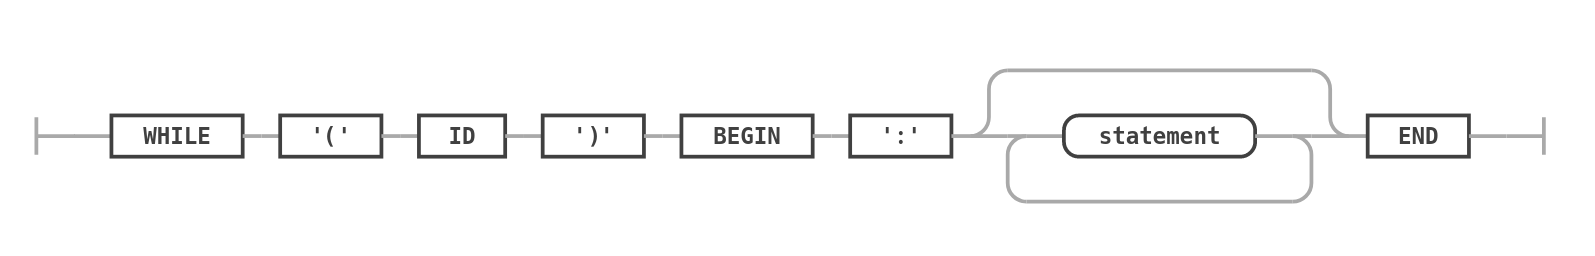
\includegraphics[width=14cm]{content/pictures/while.png}
	\caption{Die Grammatikregel für eine while-Schleife}
	\label{pic:WhileRegelWhile}
\end{figure}



\begin{figure}[h!]
	%\includegraphics[width=1\textwidth]{content/pictures/LoRaWAN-OSI.JPG}
	\centering
	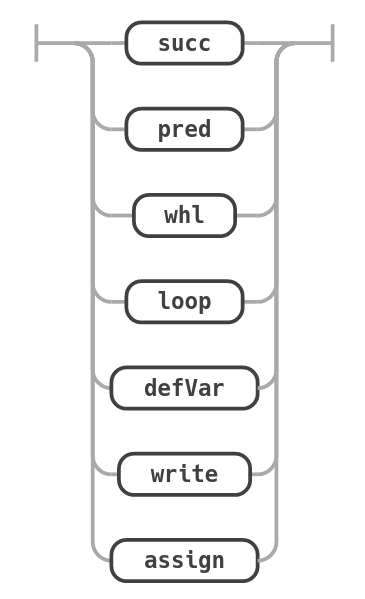
\includegraphics[width=4cm]{content/pictures/statement.png}
	\caption{Die Grammatikregel für ein Statement}
	%	\source{\cite[S. 5]{SemtechCorporation.2020}}
	\label{pic:WhileRegelStatement}
\end{figure}

Wenn ein Programm einer Menge von Grammatikregeln entspricht, bedeutet das nicht zwingend, dass der Programmcode fehlerfrei ist. Es existieren Fehleingaben, welche nur schwer durch Grammatikregeln erkannt werden können. Beispielsweise erlaubt die oben gezeigte Grammatik eine Wertzuweisung, ohne vorauszusetzen, dass die entsprechende Variable zuvor definiert wurde. Um solche Fehler zu erkennen, wird eine sogenannte semantische Analyse durchgeführt. Dieses Thema wird in \cref{chap:semantic} behandelt.

Wie ein Statement definiert wird, ist in \cref{pic:WhileRegelStatement} zu erkennen. Als Statement werden viele unterschiedliche Konzepte bezeichnet: ein \textbf{succ} und \textbf{pred} sind Statements oder auch \textbf{while} und \textbf{loop}. Aus den beiden Diagrammen lässt sich schließen, dass die Sprache auch Schleifen innerhalb von While-Schleifen erlaubt, was auch der Fall ist.


